
%%%%%%%%%%%%%%%%%%%%%%%%%%%%%%%%%%%%%%%%%%%%%%%%%%%%%%%%%%%%%%%%%%%%%%%%%%%%%%%
%
%  EGSnrc dosxyz_show manual
%  Copyright (C) 2015 National Research Council Canada
%
%  This file is part of EGSnrc.
%
%  EGSnrc is free software: you can redistribute it and/or modify it under
%  the terms of the GNU Affero General Public License as published by the
%  Free Software Foundation, either version 3 of the License, or (at your
%  option) any later version.
%
%  EGSnrc is distributed in the hope that it will be useful, but WITHOUT ANY
%  WARRANTY; without even the implied warranty of MERCHANTABILITY or FITNESS
%  FOR A PARTICULAR PURPOSE.  See the GNU Affero General Public License for
%  more details.
%
%  You should have received a copy of the GNU Affero General Public License
%  along with EGSnrc. If not, see <http://www.gnu.org/licenses/>.
%
%%%%%%%%%%%%%%%%%%%%%%%%%%%%%%%%%%%%%%%%%%%%%%%%%%%%%%%%%%%%%%%%%%%%%%%%%%%%%%%
%
%  Authors:         Iwan Kawrakow, 1998
%
%  Contributors:    Blake Walters
%
%%%%%%%%%%%%%%%%%%%%%%%%%%%%%%%%%%%%%%%%%%%%%%%%%%%%%%%%%%%%%%%%%%%%%%%%%%%%%%%


\documentclass[12pt]{article}

%
\setlength{\textwidth}{16.51cm}
%\setlength{\textheight}{23.2cm}
\setlength{\textheight}{23.5cm}
\setlength{\oddsidemargin}{0.0in}
\setlength{\evensidemargin}{0.0in}
\setlength{\topmargin}{-1.5cm}
\setlength{\parindent}{1.5em}
\setlength{\topsep}{0ex}
\setlength{\itemsep}{0ex}

\newcommand{\Co}{$^{60}$Co}
\newcommand{\parsp}{~\hspace*{1.5em}}
\setlength{\parskip}{0.1in}
\newcommand{\head}[1]{\begin{center}\begin{Large}{\bf #1}
                                              \end{Large}\end{center}}
\newcommand{\cen}[1]{\begin{center} #1 \end{center}                   }
\newcommand{\cm}{component module}
%\newcommand{\$CMNAME}{\verb+$CMNAME+}   %if already in a verbatim, wont have \
%\newcommand{MORTRAN}{\verb+MORTRAN+}
\newcommand{\CM}{Component module}
\newcommand{\etal}{{\em et.al.}}
\newcommand{\ie}{{\em i.e.}}
\newcommand{\etc}{{\em etc.}}
\newcommand{\viz}{{\em viz.}}
\newcommand{\eg}{{\em eg.}}

\renewcommand{\refname}{}

\usepackage{epsfig}


\usepackage{fancyhdr}
\renewcommand{\footrulewidth}{0.4pt}
\renewcommand{\headrulewidth}{0.4pt}


%\lhead[{\sffamily \thepage}]{{\sffamily dosxyz\_show Users Manual}}
\lhead[{\sffamily \thepage}]{{\sffamily {\tt dosxyz\_show} manual}}
\rhead[{\sffamily NRCC Report PIRS-0624}]{{\sffamily ~\thepage}}
\rfoot[{\sffamily {\rightmark}}]{{\sffamily {\rightmark}}}
\lfoot[{\sffamily {\leftmark}}]{{\small Last edited $Date: 2013/03/29 15:20:21 $}}
\cfoot{}


\usepackage{html}
\begin{latexonly}
\typeout{***Have turned off overfull and underfull messages****}
\tolerance=10000        %suppress Overfull only
\hbadness=10000         %suppress Overfull and Underfull for text (horizontal)
\vbadness=10000         %suppress Overfull and Underfull for vertical "boxes"
\end{latexonly}

\pagestyle{fancy}
\pagenumbering{arabic}

\begin{document}

\pagestyle{empty}

%\begin{flushleft}
\begin{center}

%\begin{Large}
%The dose visualization tool {\tt dosxyz\_show}\\
%\end{Large}
{\sffamily \bfseries \Huge The dose visualization tool {\tt dosxyz\_show}
\vspace{5mm}\\}
\begin{large}
I.~Kawrakow \\
\end{large}
Ionizing Radiation Standards\\
National Research Council of Canada
\\Ottawa, K1A OR6\\

Printed: \today
\\
%\hfill
\vspace{5mm}
\mbox{}\hfill NRCC Report {\sf PIRS-0624}\\

%\maketitle
\vspace{1cm}

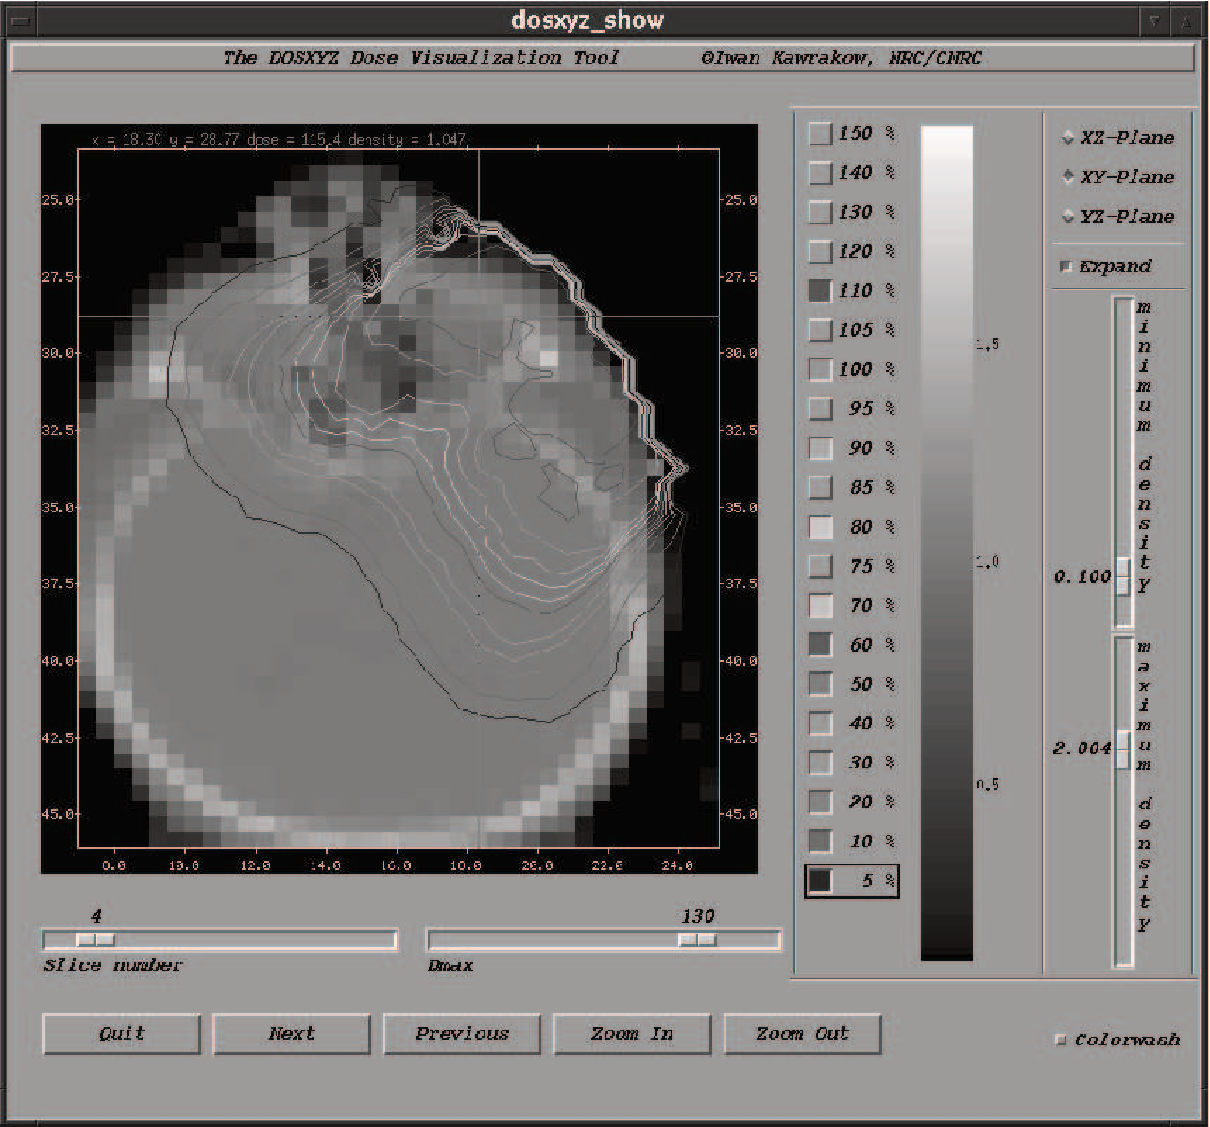
\includegraphics[height=14cm,width=16cm]{figures/dosxyz_show}


\vfill
\copyright NRC Canada, 2015
\end{center}

\newpage

\pagestyle{fancy}
\pagenumbering{arabic}
\setcounter{page}{2}

\section{\sffamily Short description}


{\tt dosxyz\_show} is a slightly modified version of
{\tt vmc\_show}, a small utility program from the
{\tt VMC} distribution,
adapted to work with the {\tt DOSXYZ}
CT data and dose formats. It displays dose
isolines on top of the corresponding CT data.
{\tt dosxyz\_show} is a public domain software distributed under the
terms of the GNU Affero General Public Licence 3.0. It was included as part
of the BEAM distribution starting in 1998.

\noindent
Note that {\tt dosxyz\_show} does not run on Windows.


\section{\sffamily Compiling and running}

The program is written in C using the OSF Motif widget
set and consists of a single file, {\tt dosxyz\_show.c}.
If you don't have Motif installed on your system, you
can use LessTif, a public domain implementation of
Motif which is relatively easy to install. To compile the
code, type
\begin{flushleft}
{\tt cc -o dosxyz\_show [preprocessor options] dosxyz\_show.c -lXm -lXt -lX11
-lm}
\end{flushleft}
Note that the order of the libraries is important.
The preprocessor options available will be described below.
If you use LessTif and have not installed the {\tt Xm} library on
the system area, you must specify the path where the library is
installed with the {\tt -L} option, {e.g.}
\begin{flushleft}
{\tt cc -o dosxyz\_show ... -L\$HOME/lesstif/lib}
\end{flushleft}
On the NRC system, the X toolkit and X11 libraries are
in {\tt /usr/X11R6/lib} and therefore {\tt -L/usr/X11R6/lib} must
be added to the compiler options.

\noindent
To run the code, type
\begin{flushleft}
{\tt dosxyz\_show CT\_file [dose\_file]}
\end{flushleft}
Here, {\tt CT\_file} and {\tt dose\_file} are the names of
the CT data file and 3D dose distribution file, both in
{\tt DOSXYZ} format. If no file extensions are specified
({\tt .egs4phant} and {\tt .3ddose}), they will be automatically
appended to the names.
Note that {\tt dosxyz\_show} expects at least one argument
(the CT data file), otherwise it will stop. The dose file
argument is optional. As there is no default directory
for the CT data files, {\tt CT\_file} must
contain the absolute path if not in the working directory.
If not found in the working directory, the dose file is assumed to
be in {\tt \$HOME/egs4/dosxyz}.

By default, the colors for the isolines are uniformly distributed
along the hue co-ordinate in the TekHVC color space (see
{\em e.g.} Adrian Nye, Xlib Programming Manual, O'Reilly \& Associates, Inc.,
for a short description of various color representations) and
should be device independent. However, it seems that there
is a bug in the Linux implementation of TekHVC and so
the resulting isoline colors differ from those on other systems.
Therefore, a RGB representation of isoline colors was
implemented which can be put into effect by
using {\tt -DMY\_COLOR} preprocessor option. If you
don't like the isoline colors, you can change them by
modifying some of the components of the {\tt red, green} and {\tt blue}
arrays defined at the beginning of {\tt dosxyz\_show.c}.

Another preprocessor option can be used to change the
density to gray shade conversion function. By default
(no preprocessor option specified), a linear mapping
is employed. With {\tt -DDG\_SQRT} you can turn on
square root mapping, {\em i.e.}
\begin{displaymath}
i_{\rm gray} = {\sqrt{\rho} - \sqrt{\rho_{min}} \over
\sqrt{\rho_{max}} - \sqrt{\rho_{min}}} N_{\rm gray}
\end{displaymath}
where $\rho$ is the the actual voxel density, $\rho_{min}$ and
$\rho_{max}$ the minimum and maximum density of the specified
displayable density window (see below) and $N_{\rm gray}$ the
number of gray shades allocated. Note that the
requirement $N_{\rm gray} \ge 64$ is coded so that
the program will stop if not able to allocate at least
64 gray shades (it seemed to me that it does not make sense
to try to visualize CT images with less than 64 gray shades).
%With {\tt -DDG\_POWER} a power law mapping scheme can be
%employed,
%\begin{displaymath}
%i_{\rm gray} = {\rho^\gamma - \rho_{min}^\gamma
You can implement your own density to gray conversion
function by introducing additional {\tt DensityToGray}
functions and preprocessor options.

\section{\sffamily Functionality}

{\tt dosxyz\_show} shows the density distribution
in a given xy-, xz- or yz-plane as a gray scale representation
together with the corresponding isoline or
color wash representation of the dose distribution
(if a {\tt .3ddose} file was specified). The isolines are
calculated using linear interpolation between the dose grid points.
Note that isolines are approximated as straight line segments in
every voxel (for efficiency). This approximation
produces good result, except in regions with sharp dose gradients
where a difference between the isoline and color was representations
might br observed.

\noindent
Note that the visualization of an arbitrary xyz-geometry
is not implemented yet but it is assumed that the planes
are distributed equidistantly (the voxel size in
a given direction is assumed to be the distance between
the second and first plane read in from the {\tt .egs4phant} file).

\noindent
\underline{\sffamily Changing the slice}
The user can change the slice by clicking on the
{\tt Next} or {\tt Previous} buttons or by using
the {\tt Slice number} scale below the viewing area.

\noindent
\underline{\sffamily Selecting the view plane}
To select the plane
(xy, xz or yz) to be shown in the viewing area, click
on the corresponding radio button in the upper-right part
of the {\tt dosxyz\_show} window.

\noindent
\underline{\sffamily Zoom in}
To use the zoom in function, click on
the {\tt ZoomIn}-button, position the mouse pointer on
the upper left corner of the image portion that you want to
zoom in and click the left mouse button, then move the
mouse until the rectangle that appears encloses the desired
image portion and click again the left button.

\noindent
\underline{\sffamily Zoom out}
To return to
the original image size simply press the {\tt ZoomOut} button.

\noindent
\underline{\sffamily Dose normalization}
When the dose array is read in, the data is normalized
to 100\% for the global dose maximum. This normalization
can be changed with the {\tt Dmax} scale below the viewing area.

\noindent
\underline{\sffamily Isoline levels}
The display of a given contour level can be switched on and off by
clicking on the corresponding toggle button right of the viewing
area. If you wish to change the set of switched on isolines at
start time, search for the boolean array {\tt set\_isolines} in
{\tt dosxyz\_show.c} and edit it according to your needs.

\noindent
\underline{\sffamily Density range}
The {\tt minimum density} and {\tt maximum density} scales
can be used to define the displayable density range.

\noindent
\underline{\sffamily Image expansion}
When the {\tt Expand}-button is on, the image is expanded to
fill the entire viewing area which may lead to a different
length scale (cm per pixel) in x- and y-direction. If you
wish to have the same length scale in x- and y-direction, simply
switch off the {\tt Expand}-button (when {\tt Expand} is deactivated,
only square image portions can be selected with the zoom in function).

\noindent
\underline{\sffamily Point dose values}
There are two ways to obtain point dose values: (i) Go to the
point of interest with the mouse and click the left button.
The dose value at this point will appear on the screen;
(ii) Place the mouse pointer in the viewing area and click the
right button activating in this way the {\tt GetDose} function.
{\tt GetDose} shows a cross hair which follows the mouse motions
and prints the corresponding co-ordinates, dose and density
values in the upper portion of the viewing area. {\tt GetDose} is
deactivated by clicking the middle mouse button or leaving
the viewing area.

\noindent
\underline{\sffamily Color wash representation}
A color wash
representation of the dose distribution
can be switched on with the {\tt Colorwash} button
(note, however, that method (i) for point dose does not
produce very good results with color wash on).

\section{\sffamily Resources}

Contrary to the recommendations of all Motif manuals to
specify widget resources (font, colors, geometry etc.) in a
resources file ({\tt .Xdefaults} or the application-defaults file),
I have hard coded most of the resources to avoid dealing
with various, possibly difficult to handle, user settings.

\end{document}
